\chapter*{Introduction / Motivation (3 pgs)}
\addcontentsline{toc}{chapter}{Introduction}

	liquid helium discovery, 1908, Heike Onnes, liquid state at 4.2K, superfluid state below 2.17K, full phase diagram:

	\begin{figure}[h]
		\centering
		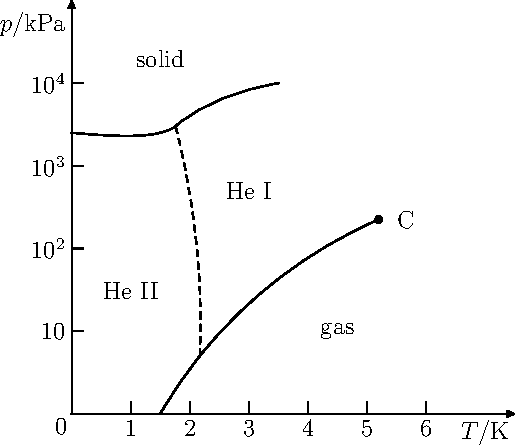
\includegraphics[width=0.5\textwidth]{graphics/phase_diag}
		\caption{p-T diagram}
		\label{phase}
	\end{figure}

	labelling He-I, He-II, no solid state at 0K (weak van der Waals), only at 2.5MPa

	strange properties, thermal conductivity, negligible viscosity through capillaries

	Landau, Tisza: phenomenology, two-fluid model, proved bz rotating discs:

	\begin{figure}[h]
		\centering
		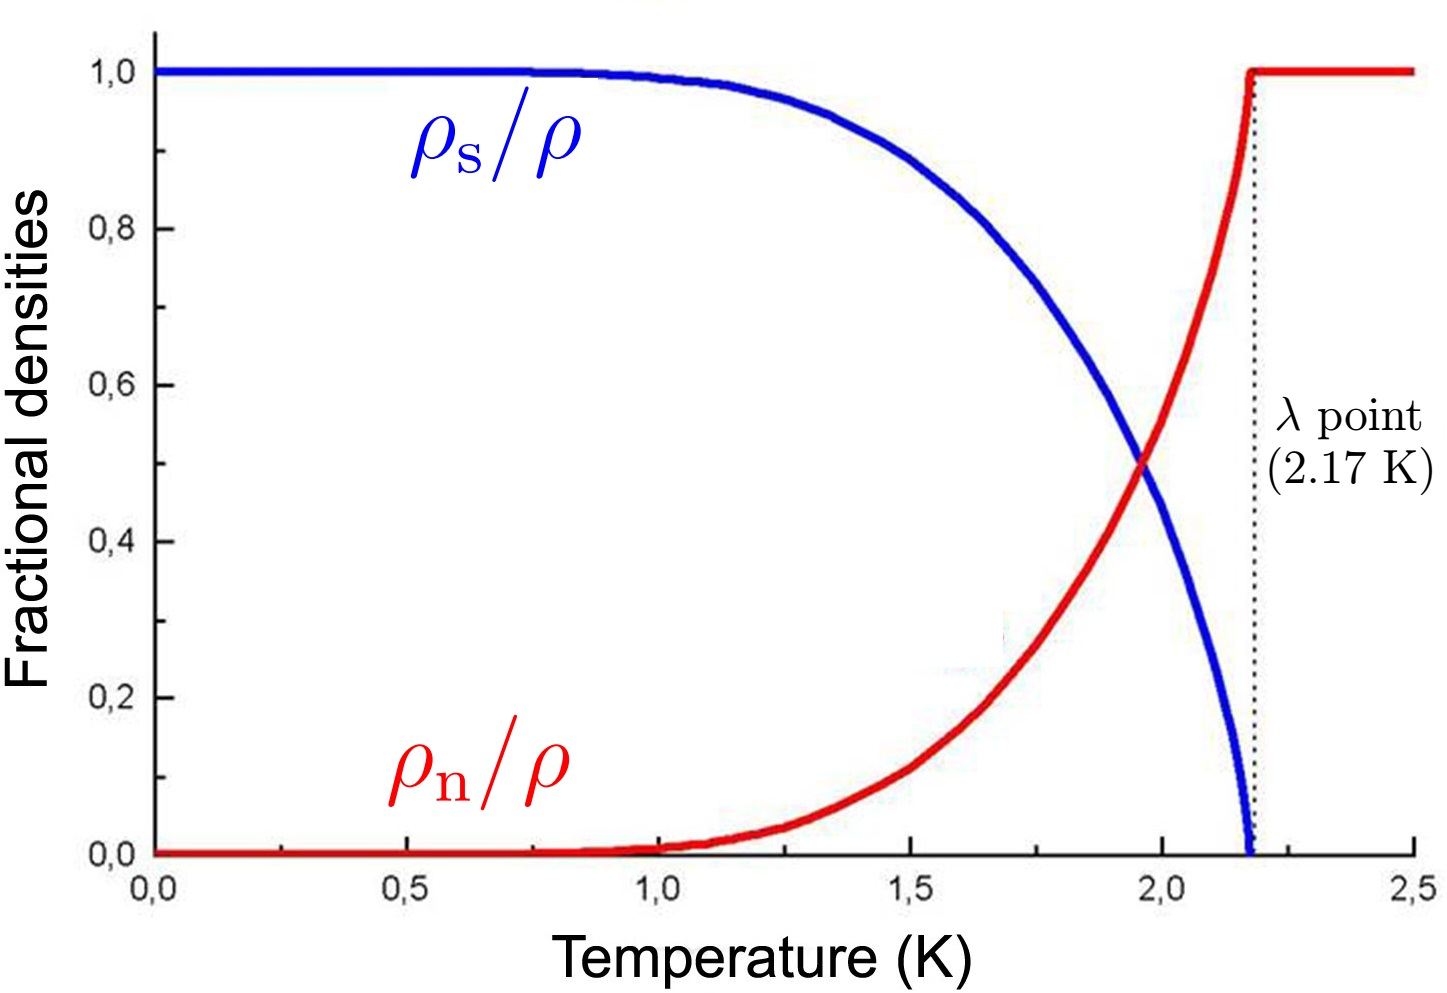
\includegraphics[width=0.5\textwidth]{graphics/densities}
		\caption{temperature dependence of densities}
		\label{densities}
	\end{figure}

	London: similarity of superfluid component with orbiting electorns, macroscopic wave func

	irrotational fluid, quantum vortices, tangle:

	\begin{figure}[h]
		\centering
		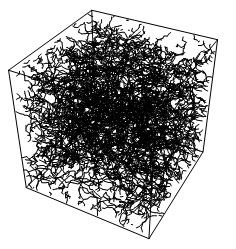
\includegraphics[width=0.5\textwidth]{graphics/QT-tangle}
		\caption{Quantum Turbulence}
		\label{QT}
	\end{figure}

	CT experiments: transition to turbulence, drag coeffs

	QT experiments: coflow, counterflow, second sound

	QT vs CT: complicated N-S equations, critical velocity or Reynolds number, QT has probably more critical velocities

	Simulations: filament model, boundaries

	Motivations: investigate critical velocities and vortex density, create numeric model

	Goals: measure hydrodynamic profiles for more temperatures with oscillating object, transition from CT to QT, investifate numerically vortex rings

\newpage
\chapter{Theoretical Background (15 pgs)}

The theoretical part of this Thesis is composed of two chapters:

\begin{itemize}
	\item[1.] Mesoscopic view - theoretically cover London's theory, creation and numerical modelling of quantum vortex, vortex dynamics.

	\item[3.] Macroscopic view - hydrodynamics of two-fluid model, oscillatory motion in such fluid, creation of QT, existence and usage of second sound

\end{itemize}

Many of this is covered in textbooks and papers.

He properties, total spin, Bose gas, critical temperature, heat capacity

\newpage

{\Huge \bfseries Mesoscopic view}
\addcontentsline{toc}{chapter}{Mesoscopic model}
\vspace{0.3cm}

\section{London's theory}
\begin{itemize}
	\item London's theory
	\item NLSE (Schr eq)
	\item macroscopic wave function
	\item no vorticity
	\item quantized circulation
\end{itemize}

\section{Quantum vortex}
\begin{itemize}
	\item definition
	\item induced velocity
	\item energy
	\item quantized circulation
	\item quantum turbulence
\end{itemize}

\section{Vortex filament model}
\begin{itemize}
	\item graph model
	\item state definition
	\item curve coordinates
	\item derivatives
	\item self-induced velocity
	\item LIA approximation
\end{itemize}

\section{Vortex dynamics}
\begin{itemize}
	\item magnus force
	\item mutual friction
	\item Schwarz's equation
	\item special case - quantum ring (properties)
	\item Kelvis waves (?)
\end{itemize}

\newpage

{\Huge \bfseries Macroscopic view}
\addcontentsline{toc}{chapter}{Macroscopic model}
\vspace{0.3cm}

\section{Hydrodynamics of two-fluid}
\begin{itemize}
	\item Landau's assumptions
	\item two densities, velocities (+pic)
	\item updated hydrodynamical equations - HVBK
	\item dynamical similarity
	\item Reynolds number
\end{itemize}

\section{Oscillatory motion in superfluid}
\begin{itemize}
	\item penetration depth
	\item Re for oscillations
	\item defining depth and Re separately for normal and superfluid components
\end{itemize}

\section{Quantum turbulence}
\begin{itemize}
	\item critical velocity according to landau
	\item critical velocity scaling in oscillatory case
	\item T dependence of critical velocities (Bc. results)
\end{itemize}

\section{Second sound}
\begin{itemize}
	\item what it is
	\item velocity of second sound
	\item attenuation
	\item vortex line density estimate
\end{itemize}

\newpage
